\documentclass[11pt,a4paper,twoside]{thesis}

\usepackage{graphicx}
\usepackage[utf8]{inputenc}
\usepackage[spanish]{babel}
\usepackage[left=3cm,right=3cm,bottom=3.5cm,top=3.5cm]{geometry}
\usepackage{titlesec}
\usepackage{listings}
\usepackage{xcolor}
\usepackage{hyperref}
\usepackage{amsmath}
\usepackage{amssymb}
\usepackage[utf8]{inputenc}
\usepackage{enumitem}
\usepackage{booktabs}

\begin{document}

%%%% CARATULA

\def\autor{Adrian Norberto Marino}
\def\tituloTesis{Trabajo práctico 2: Búsqueda bibliografica}
\def\runtitulo{Resumen}
\def\runtitle{Trabajo práctico 2: Búqueda bibliografica}

%\def\director{Obi-Wan Kenobi}
%\def\codirector{Master Yoda}

\def\lugar{Buenos Aires, 2023}

% -----------------------------------------------------------------------------
% Caratula,  Resumen, agradecimientos y dedicatoria.
% -----------------------------------------------------------------------------
\newcommand{\HRule}{\rule{\linewidth}{0.2mm}}
%
\thispagestyle{empty}

\begin{center}\leavevmode

\vspace{-2cm}

\begin{tabular}{l}

\includegraphics[width=3.6cm]{./images/logouba.png}
\end{tabular}


{\large \sc Universidad de Buenos Aires\\Facultad de Ciencias Exactas y Naturales \\ Facultad de Ingeniería}

\vspace{6.0cm}

\vspace{3.0cm}
%{
%\Large \color{red}
%\begin{tabular}{|p{2cm}cp{2cm}|}
%\hline
%& Pre-Final Version: \today &\\
%\hline
%\end{tabular}
%}
%\vspace{2.5cm}

\begin{huge}
\textbf{\tituloTesis}
\end{huge}

\vspace{2cm}

{\large Trabajo Final de la \textit{Especialización en Explotación de Datos y Descubrimiento del Conocimiento}}
\vspace{2cm}

{\large \href{https://github.com/adrianmarino/thesis-paper}{Github Project}}

\vspace{2cm}

{\Large \autor}

\end{center}

\vfill

{\large

%{Director: \director}

\vspace{.2cm}

%{Codirector: \codirector}

\vspace{.2cm}

\lugar
}

\newpage\thispagestyle{empty}

%
\frontmatter
\pagestyle{empty}
% -----------------------------------------------------------------------------
%
%
%
%\cleardoublepage
\tableofcontents
%
%
\mainmatter
\pagestyle{headings}
%
%
%
%
% -----------------------------------------------------------------------------
% Contenido de la tesis
% -----------------------------------------------------------------------------

\setitemize{itemsep=0.5pt}

\chapter{Introducción}

Los sistemas de recomendación tienen como objetivo principal proporcionar a los
usuarios productos, promociones y contenidos relevantes a sus preferencias o
necesidades. Estos sistemas permiten a los usuarios encontrar de forma ágil y
eficiente lo que están buscando. Formalizando esta definición, podemos decir
que los sistemas de recomendación buscan ayudar a un usuario o grupo de
usuarios a descubrir ítems que se ajusten a sus preferencias, dado un conjunto
de ítems que puede ser extenso o un amplio espacio de búsqueda.

\begin{sloppypar}
	Este objetivo puede variar dependiendo de cada negocio: Si consideramos un
	\textit{e-commerce} de \textit{delivery} gastronómico, su propósito sería
	ofrecer a los clientes platos relevantes a un precio asequible y con un tiempo
	de entrega aceptable.
\end{sloppypar}

Si hablamos de un \textit{e-commerce} de productos, su objetivo consiste en
proporcionar a los usuarios aquellos productos que satisfacen sus necesidades,
a un precio que estén dispuestos a pagar. Además, se busca garantizar una
experiencia satisfactoria con los vendedores.

En el negocio de visualización de contenido (audio, video, texto, etc..), el
objetivo es acercar a sus usuarios contenido a fin a sus preferencias para
mejorar su experiencia en la plataforma.

El objetivo principal en todos los casos es mejorar la conversión. En el campo
del \textit{marketing}, se define la conversión como las acciones realizadas
por los usuarios que están alineadas con los objetivos de la empresa. Por
ejemplo, aumentar el volumen de compras en un \textit{e-commerce} de productos,
incrementar la cantidad de entregas mensuales en un \textit{e-commerce} de
\textit{delivery} gastronómico, aumentar las impresiones de publicidad en
aplicaciones de visualización de contenido, prolongar el tiempo de permanencia
en plataformas de \textit{streaming} de audio o video, entre otros. Existen
numerosos ejemplos en los que el objetivo común es mejorar la conversión y el
compromiso del usuario con la marca, es decir, el \textit{engagement}.

Desde un enfoque técnico, los sistemas de recomendación se utilizan para
predecir el grado de preferencia de un usuario con un artículo específico. Esto
se logra aplicando algoritmos de optimización que minimizan la diferencia entre
el grado de preferencia esperado y el grado de preferencia real del usuario.
También existen otros enfoques que utilizan medidas de distancia para
determinar este grado de preferencia. En secciones posteriores, exploraremos
estos conceptos con mayor detalle.

\clearpage
\section{Tipos de sistemas de recomendación}

A continuación, en la figura~\ref{fig:clasification}, se pueden observar las
diferentes categorías y sub-categorías de los sistemas de recomendación:

\begin{figure}[!htb]
	\centering
	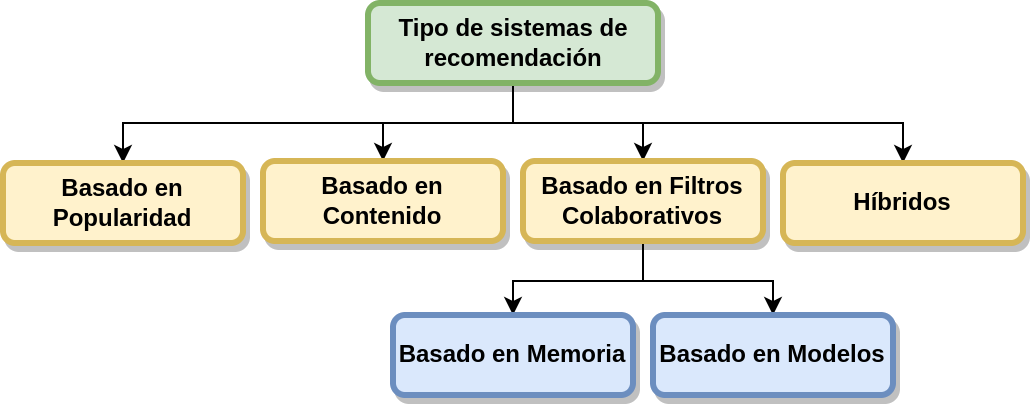
\includegraphics[width=12cm]{./images/clasificacion-sis-rec.png}
	\caption{Clasificación de tipos de sistemas de recomendaciones.}
	\label{fig:clasification}
\end{figure}

\subsection{Basados en Popularidad}

Este tipo de sistema de recomendación utiliza alguna característica de
popularidad de los ítems en cuestión. Algunos ejemplos de estas características
podría ser la cantidad de vistas, la cantidad de compras o la cantidad de
comentarios positivos, o una combinación de ellas. Luego, estos sistemas buscan
los K elementos más populares. Si bien este tipo de enfoque proporciona buenos
resultados para nuevos usuarios, sus recomendaciones no tienen en cuenta las
preferencias individuales de cada usuario, ya que se basan en estadísticas
comunes a todos los usuarios. Por esta razón, a menudo no se consideran
sistemas de recomendación en sentido estricto. No obstante, siguen siendo
ampliamente utilizados debido a su capacidad para generar una alta tasa de
conversión, a pesar de la falta de personalización.

\subsection{Basados en Contenido}

Este tipo de sistema de recomendación necesita un trabajo previo de ingeniería
de \textit{features} sobre los ítems. Se busca definir cuales son los
\textit{features} mas significativos para la tarea en cuestión, y cual es el
grado de adecuación de cada ítems a los \textit{features} seleccionados.

Por otro lado, existen dos formas de utilizas estos modelos:

\begin{itemize}
	\item El usuario esta registardo pero no realizo interacciones con los ítems: Este
	      escenario se da con usuarios que se registraron pero aun no han calificado
	      ningun ítems. En estos casos muchas aplicaciones optan por realizar un encuetra
	      inicial. Esta encuentra se utiliza para consutar al usuario \textit{features}
	      reelevantas que permitiran comenzar a realizar recomendaciones. Por ejemplo, se
	      podria presentan una lista de géneros, actores, directores, etc. Luego, el
	      usuario realiza un apuntuación de acuerdo al su nivel de gusto. Estas encuentas
	      se suelen realizar cada cierto tiempo, dadoq ue hay usuarios que tinene una
	      frecuencia muy baja de interacicon con el sistema.
	\item El usaurio se registro hace un tiempo y tiene cirta frecuencia de interacciones
	      con los ítems: En esta caso, se utilizan las clasificaciones del usuario sobre
	      para realizar las recomendaciones. Este enfoque suele tener mejores resultados,
	      ya que muchas veces (dependiendo del dominio de las recomendaciones) el usuario
	      no conoce inicialmente que es lo que le gusta o bien puede cambiar de pareser
	      en sus opiniones. En comparación este enfoqeu es mejor al enfoque anterior,
	      dadoq ue el modelo tiene un concimiento mas acutalizado sobre los gustos del
	      usuario, permitendo realiazr recomendaciones mas alineadas a los gustos del
	      usaurio.
\end{itemize}

Ambos emfoques puede combinarse. Supongamos que el cientifico de dados
seleciona los generos como \textit{features}. Inicialmente peude realizar una
encueta y conocer el gradode gusta del usuario por cada genero. Luego el
usaurio coomenxa a calificar items. Estoa valores ahora pueden actualizarse
utilizando alguna medida a aprtir de las calificaciones. De esta forman se
podrian utilizar como enfoques complementarios.

Dadas estas interacciones de los usuarios, se puede definir el grado de
preferencia de los usuarios a cada \textit{feature} definido para los ítems.
Con esta información, es posible encontrar tanto ítems como usuarios similares
y realizar recomendaciones del tipo:

\begin{itemize}
	\item Para el \textit{Usuario A} el cual tiene ciertos niveles de preferencia por
	      cada \textit{features}, se pueden recomendar los \textit{Ítem X} e \textit{Ítem
		      Y}. El modelo puede infererir el grado de preferencia del \textit{Usuario A}
	      para cada item existente y luego ordenarlos. En este caso, el \textit{Ítem X}
	      es de mayor preferencia para el usaurio que el \textit{Ítem Y}.

	\item Dado el \textit{Usuario A}, el cual tiene preferencia por el \textit{Ítem X},
	      también podría tener preferencia por el \textit{Ítem Y}, por ser muy cercano o
	      similar al \textit{Ítem X}.

	\item Dos \textit{Usuarios A y B} cercanos o similares, tendrán preferencias
	      similares. De esta forma es posible recomendar ítem consumidos por el
	      \textit{Usuario A} al \textit{Usuario B} y vise versa.
\end{itemize}

La principal desventaja de este enfoque, es la necesidad de realizar ingeniería
de \textit{features} para encontrar los \textit{features} que produzcan
recomendaciones relevantes al usuario. El modelo no encuentra estos
\textit{features} automáticamente, sino que deben ser definidos de antemano
manualmente. Se puede apreciar que esto introduce un sesgo al momento de
seleccionar los \textit{features} o construirlos en base a datos referentes a
los ítems. Como ventaja, si se encuentran los \textit{features} correctos se
pueden lograr muy buenos resultados.

\subsection{Basados en Filtrado Colaborativos}

Estos modelos, a diferencia de los modelos basados en contenido, no requirieren
ingeniería de \textit{features}, lo que hace muy simple su implementación, ya
que únicamente es necesario registrar las interacciones de los usuarios para
con los ítems. Luego, el propio modelo encuentra automáticamente los
\textit{features} mas relevantes dependiendo de la cantidad de columnas que se
especifiquen (dimensiones de un vector \textit{Embedding}). Ejemplos de
interacciones podrían ser:

\begin{itemize}
	\item El \textit{Usuario A} visualizo el \textit{Ítem X} el dia 2 de marzo de 2022.
	\item El \textit{Usuario A} compro el \textit{Ítem X} el dia 10 de marzo de 2022.
	\item El \textit{Usuario A} califico al \textit{Ítem X} con 5 puntos el dia 25 de
	      marzo de 2022.
\end{itemize}

Ambos tipo de modelos, basados en contenido y filtros colaborativos,
personalizan sus recomendaciones. Es decir, ajustan las recomendaciones a las
preferencias de cada usuario particular. Además, ambos permiten encontrar
usuarios e ítems similares y recomendar ítems entre usuarios similares.

Por otro lado, los modelos basados en filtros colaborativos, descubren un
espacio latente de soluciones sin necesidad de recolectar datos y definir
\textit{features} en forma manual, a diferencia de los modelos basados en
contenido. La selección o construcción manual de \textit{features} puede llevar
a una solución sesgada, ya que no esta basada en datos sino en el juicio
experto del científico de datos. Esto puede llevar a una selección subjetiva de
los \textit{features} que se aleje de la realidad, introduciendo un sesgo en la
predicción.

No todo son rosas con estos modelos, dado que sufren un problema llamado
\textit{Cold start} o arranque en frio. Los usuarios nuevos son aquellos que
aun no han realizado ninguna interacción con el sistema. Estos modelos no
podrán realizar recomendaciones a estos usuarios, dado que requieren un mínimo
de interacciones para comenzar a ofrecer recomendaciones con cierta precisión.

Además, existen otros problemas referidos al cambiar la cantidad de
interacciones de los usuarios. Si pensamos en una solución donde alimentamos al
modelo con una ventana de interacciones para los últimos N meses, tendremos las
siguiente situaciones:

\begin{itemize}
	\item Usuarios nuevos: Los usuarios nuevos no tendrán interacciones. Por lo tanto,
	      este modelo no podrá realizar ninguna recomendación. En general, se establece
	      un mínimo de interacciones para que el modelo pueda realizar recomendaciones de
	      forma acertada.
	\item Usuarios con pocas interacciones: Por otro lado, tenemos a los usuarios que
	      tienen una baja taza de interacciones con el sistema o aplicación. Por ejemplo,
	      en un \textit{e-commerce} de venta de productos, hay usuarios que compran con
	      mucha frecuencia y otros muy de vez en cuando. Estos últimos, en general
	      tendrán una baja taza de interacción pudiendo caer por debajo del umbral mínimo
	      que requiere el modelo. De esta forma, tendremos usuarios que quedarán fuera
	      del modelo actual.
	\item Usuarios con muchas interacciones: En este caso, el usuario tiene una gran
	      cantidad de interacciones con ítems. Para estos usuarios, el modelo podrá
	      ofrecer recomendaciones relevantes, ya que cuanto mas interacciones se tenga,
	      el modelo se ajusta con mas facilidad a sus preferencias. Por otro lado, esto
	      puede ser una gran desventaja, ya que se produce un efecto de túnel. Es decir,
	      el usuario obtiene recomendaciones muy ajustadas a sus preferencias, perdiendo
	      la capacidad de descubrir nuevos ítems que podrían ser relevantes. Por esta
	      cuestión se suelen mezclar tanto recomendaciones personalizadas como
	      no-personalizadas, para favorecer el descubrimiento de nuevos ítems.

\end{itemize}

\subsection{Categorías dentro de los modelos basados en filtros colaborativos}

Dentro de los sistemas de recomendación basados en filtros colaborativos,
tenemos dos sub-clasificaciones referidas a la forma en la que se realizan las
predicciones.

\subsubsection{Basados en Memoria}

Este tipo de modelos, como su nombre lo indica, mantiene sus datos en memoria.
Se recorren todos los datos (\textit{full scan}) cada vez que se necesita
realizar un inferencia o predicción (fijando un número de vecinos a comparar).
Un ejemplo de estos modelos es el algoritmo de k vecinos cercanos
(\textit{KNN}), el cual mantiene una matriz rala de distancias en memoria, la
cual se recorre completamente para comparar las distancias entre filas o
columnas, usando alguna medida de distancia como puede ser la \textit{distancia
	coseno}, \textit{coseno ajustada}, \textit{manhattan}, etc.. Para mitigar el
problema de búsqueda exhaustiva (\textit{full scan}), se puede utilizar una
memoria \textit{cache} y asi realizar estas búsquedas una única vez. Otro
problema es su limitación al tamaño máximo de la memoria con la que se cuenta,
es decir, que el tamaño de la matriz depende de la memoria máxima disponible.
Esto puede mitigarse utilizando implementaciones de matrices rala, las cuales
comprimen los datos en memoria guardando unicamente las celdas que tienen
datos. Además, es posible utilizar un memoria \textit{cache} que mantenga en
memoria las búsqueda mas frecuentes y baje a almacenamiento secundario las
menos frecuentes. Todos estos problemas de \textit{performance} y uso de
recursos se deben a que \textit{KNN} no reduce la dimensionalidad de los datos,
como si lo hacen varias implementaciones basadas en \textit{embeddings},
\textit{auto-encoder}, redes neuronales etc.., donde lo que se busca una
representación mas compacta de los ítems y usuarios sin perder información. Mas
allá de estos problemas, los resultados obtenidos por estos modelos no están
muy alejados de aquellos que se encuentran en el estado del arte. Puede
recomendarse su uso cuando tenemos un dominio reducido, dada su simplicidad.

\subsubsection{Basados en Modelos}

Algunos ejemplos de estos modelos son los clasificadores bayesianos, redes
neuronales, algoritmos genéticos, sistemas difusos y la técnica de
descomposición matricial (\textit{SVD}). Estos modelos en general buscan
directa o indirectamente reducir la dimensionalidad de los datos. De esta
forma, es posible utilizarlos en dominios con una gran cantidad de datos.

\clearpage
\subsection{Modelos Híbridos o Ensambles}

Son aquellos modelos que combinan mas de una técnica de recomendación, también
llamados ensambles de modelos.

Comunmente se utilizan para resolver el problema de \textit{Cold start} o
arranque en frio que sufren los modelos de recomendación basados en filtros
colaborativos.

Los modelos de recomendación colaborativos, no puede realizar recomendaciones a
usuarios que aun no han calificado ítems. Para soplucinar esta probleamtica se
utilizan modelos de recomendación que no dependen de las interacciones solo con
estos usuarios solucionando parcialmente el problema de \textit{Cold start} o
arranque en frio. Exiten distinto enfoques que permite abordar este problema.
Los ensambles solucionan ese problema y al mismo tiempo puede realizar
recomendaciones con mayor exactitud que las que puede realizara cada modelo por
separado. Por otro ladu utilizar ensample no asegura una mejora en las
recomendaciones, ya qeu es algo muy dependiende te los datos, de la
heterogeneidad de los modelos y de la técnica de ensamblado que se utilice.

\subsection{Estrategias de ensamble de modelos}

A continuación se definen las estrategias de ensamble mas comunes:

\subsubsection{Switching}

Esta técnica consta de realizar un intercambio de los modelso de recomendacion
dependiendo de la cantidad de interaccioens con las que cuente el usuario. Es
una buena práctica tomar una un periodo de N horas, días o meses para calcular
el número de interacciones. Un ejemplo podria ser:

\begin{itemize}
	\item Si el usuario tiene menos de N interacciones, se utiliza un recomendador por
	      pupuladidad.
	\item Si el usuario tiene enter 5 y 10 interacciones, se utiliza un recomendador
	      basado en contenido.
	\item Si el usuario tiene mas de 20 interaccione, se utiliza un recomendador basado
	      en contenido.
\end{itemize}

El proncipal problema de este enfoque es el cambio abrupto en el patron de las
recomendaciones al cambiar de una recomendación a otro, yaque las calidad de
las recomendacion puede varias mucho, como en el caso de l ejemplo anterior.

\subsubsection{Mixing}

Esta técnica combina los ratings predichos por cada modelos de recomendacion,
para dada item recomendado. Habitualmente se realiza una normalizacion por el
rating mas alto. De esta forma cada ítem tiene un score entre 0 y 1. Donde 1 es
la puntuación más alta. Otra alternativa sería realizar un \textit{scoring} por
la media, promedio pesado, mediana de los \textit{rating} predichos por cada
modelo para cada ítem. Esta técnica puede ser mas efectiva si se aplica en
conjunto con la técnica de \textit{switching}, ya que permimite suabixar entre
enter modelos, mezclando las recomendaciones de dos modelos cunado se llega a
un rango de interacciones pre-establecido como frontera entre modelos.

\subsubsection{Weighted}

Esta técnica en un caso particular de la técnica de \textit{Mixing}. Se refiere
al caso en que se realiza un promedio pesado de los ratings predichos mor cada
modelo para el mismo ítem. Los pesos se asigna manualmente, es decir no existe
ningun proceso para optimizar o descubrir estos hiperprametros.

\subsubsection{Regresión Lineal}

Esta técnica es similar al enfoque \textit{Weighted}, pero en este caso, si se
optimizan los pesos utilizando un modelo de regresión linear. El proceso consta
de los siguietes pasos:

\begin{enumerate}
	\item Se entrena cada modelo de recomendación por separado utilizan el mismo conjunto
	      de entrenamiento y evaluación
	\item Con cada modelo se predice el \textit{rating} para todo el conjunto de
	      entrenamiento. De esta forma como resultado, se tiene un nuevo conjunto de
	      entrenamiento, donde se encuentra como columnas: usuario, item, los
	      \textit{ratings} predichos por cada modelos como columnas, y finalmente el
	      \textit{rating} real realizado por el usuario. Lomimsmo sucede con el conjunto
	      de evaluación.
	\item Finalmente, se entrena y evalua una regresión lineal como los conjuntos
	      construidos en el paso anterior.

	      A diferencia del enfoque \textit{Weighted} ahora si los pesos se ajustan de
	      acuerdo a los datos de entrenamiento.

\end{enumerate}

\subsubsection{Stacking}

El enfoque \textit{Stacking} es una genezalización del enfoque de
\textit{Regresión Lineal}. Este consta de aplicar cualquier modelo (incluido
regresion lineal) para ajustar los pesos, pudiendo de aplicar culquier modelos
linar o no linal como redes neuronales, regresiones polinomicas, etc.

\subsubsection{Feature-Weighted Linear Stacking}

Esta técnica a grandes razgos gaarda similitud con los últimos 3 métodos
expuestos (\textit{Weighted}, \textit{Regresión Lineal}, \textit{Stacking}).
Consta de aplicar un función lineal similar a una regresión, donde cada modelo
se puede pensar como una componentes de la regresión, cada una multplicada por
una meta función o función \textit{feature-weights}. Estas meta funciones
pueden ser pensadas como pesos guiados por reglas duras. Es decir, sus valores
estan pesados por reglas duras. Esta reglas ayudan a manejar el nivel de
contibución que tiene cada modelo sobre el \textit{rating} resultado de la
prediccion. Por ejemplo, podriamos utilizar reglas duras para aumentar la
contribución de un modelo basado en contenido cuando el usuario tiene pocas
interacciones o aumentar la contrucon de un modelo de filtros colaborativos
cuando el número de interacciones del usuario aumenta. En definitiva, es una
formas de realizar lo que se llama \textit{blend} o mezcla de las
construciciones de cada modelo al \textit{raging} resultado aplicando una
transición suave.

\subsubsection{K-Arm Bandit utilizando Thompson sampling}

La tecnica propuesta se basa en el conocido problema de los bandidos multi
brazo o el problema de las maquinas tragamonedas.

El problema consiste en que tenemos una cantidad K de maquinas tragamonedas y
contamos con una cantidad limitadas de fichas. Se busca producir la mayor
cantidad de ganancias y en el proceso descibrir cual es la probabilidad de
existo de cada maquina. Todo esto utilizando la menor cantidad de fichas
posible. En definitiva, se busca maximizar la ganancia descubriendo de forma
temprana las probabilidades de existo de cada maquina.

Este es un método iterativo, donde en cada iteración, el método selecciona una
máquina, realiza una jugada y registra si se ganó o se perdió.

La selección de la máquina puede ser al azar, o estar guiada por una heurística
o método estadístico.

Cuando la selección es al azar, se dice que se está en modo o etapa de
exploración, es decir, se gastan fichas para acumular resultados de cada
máquina y así registrar una serie de éxitos y pérdidas en cada máquina. Cada
máquina se puede pensar como una variable binomial, es decir toma dos valores,
gano o perdio.

Luego, con esta sucesión de eventos, se estima una distribución beta para cada
máquina y finalmente se toma una muestra de un valor de esa distribución. Este
valor sera el valor mas probable o la probabilidad de éxito de la máquina.

Ya realizada una primera etapa de exploración, en las próximas iteraciones se
puede hacer uso del conocimiento actual y seleccionar la máquina con mayor
probabilidad de éxito. A esta etapa se le llama explotación, ya que se está
explotando o haciendo uso del conocimiento aprendido con anterioridad.

El proceso realiza una mezcla de estas dos etapas de forma estocástica,
haciendo uso de la estrategia \textit{epsilon greedy} (mejorada). Esta
estrategia, elige de forma aleatoria entre ambas técnicas de selección, con una
probabilidad de exploración \textit{epsilon}. Esta probabilidad ira
disminuyendo a medida que aumenta el número de iteraciones. Esta es una mejora
que permite restringir la exploración. Tiene mucho sentido, ya que a medida que
se realizan más jugadas, se comprende más el problema y ya no es necesario
realizar una selección al azar.

En conclusión, se busca determinar la probabilidad de éxito de cada máquina,
realizando la menor cantidad de jugadas posibles.

Este enfoque se utiliza en el ámbito de sistemas de recomendación para
determinar el modelo con mayor probabilidad de éxito para cada usuario. Es
decir, cuál es el modelo que tiene mayor probabilidad de realizar una
recomendación similar a la que realizaría el usuario. Esta medición de éxito
depende de la métrica a evaluar.

A diferencia de varios de los modelos de ensamble anterioremente expuestos,
donde se requiere relizar una misma predicción para todos los modelos parte de
ensamble, este en foque realiza la predicción en un unico modelo, debido a que
es una estrategia de selección de modelos. Esto se traduce en un uso mas
eficiente de los recursos de CPU, GPU y memoria del sistema, ya que estos
modelos en general se ejecutan como servicios \textit{cloud} (en la nuve) en
\textit{AWS} (\textit{Amazon Web Services}) o \textit{GCP} (\textit{Google
	Cloud Platform}), donde se paga unicamente por el uso de recursos que relizan
los servicios o modelo en este caso.

\clearpage
\section{Descripción del problema y motivación}

Con este trabajo se busca contestar a las siguientes preguntas:

\subsection{¿Los modelos basado en filtro colaborativos que utilizan técnicos de
	\textit{Deep Learning}, obtienen mejores resultados que aquellas que no las utilizan?}

La idea detrás de esta pregunta es realizar \textit{benchmarks} sobre distintos
modelos del estado de arte basados en \textit{Deep Learning} o no, utilizando
el mismo set de datos y las mismas métricas. De esta forma, se busca comprender
cual es la diferencia en \textit{performance} entre los modelos seleccionados.
Por otro lado, se busca comprender cuando es mas adecuado utilizar cada
enfoque. Como ya se comentó en el apartado de introducción, hay modelos que
están mas limitados que otros según el número de recursos de \textit{hardware}
o interacciones con los que se cuenta.

\subsection{¿Cuáles son las ventajas y desventajas de cada enfoque a la hora de aplicar estas técnicas?}

Esta pregunta se refiere a comprender cuando es conveniente aplicar una técnica
u otra teniendo en cuenta las ventajas y desventajas de cada enfoque y modelo.

\subsection{¿Cómo se puede solucionar el problema de \textit{Cold start}
	que sufre el enfoque de recomendación basado en filtros colaborativos? (tesis)}

Como ya se comentó en la introducción, los modelos de filtro colaborativos
necesitan un número mínimo de interacciones usuario-ítem para poder operar y
producir recomendaciones aceptables. La propuesta es explorar enfoques que
permiten lidiar con este problema. Uno de los enfoques más comunes es utilizar
ensambles de modelos basados en filtros colaborativos con otros modelo basados
en contenidos o popularidad. Estos ensambles puede diferir en sus técnicas
dependiendo del dominio de los datos.

\section{Objetivos}

Como primer objetivo, se pretender comprender cuales son los fundamentos
teóricos sobre los que se apoya cada técnica aplicada y bajo que escenarios
puede ser conveniente aplicarlas. Por otro lado, se intenta determinar cual es
la diferencia en \textit{performance} de cada técnica aplicada sobre el mismo
set de datos, midiendo su \textit{performance} utilizando las mismas métricas.
¿Obtenemos diferencias significativas?

Como segundo objetivo, se busca proponer nuevas técnicas y/o explorar técnicas
existentes que permite lidiar o solucionar el problema de \textit{Cold start}
que sufren los sistemas de recomendación basados en filtros colaborativos.
Ademas, se compararan esta técnicas mediante un \textit{benchmark} propuesto,
para compara como se comporta cada modelos ante usuarios con escasas o ninguna
interacción en el set de datos propuesto.

%%%% BIBLIOGRAFÍA

% Establece el estilo de las referencias bibliográficas
% otago, plain, apa, ieee, IEEEtran, etc...
\bibliographystyle{IEEEtran}
\renewcommand{\bibname}{Referencias}
\bibliography{cites} % Especifica el nombre del archivo .bib sin la extensión .bib

\end{document}